\documentclass[a4paper, 20pt,reqno]{article}
\usepackage[left=2cm,right=2cm,top=2cm,bottom=2cm]{geometry}
\usepackage[T2A]{fontenc}
% \DeclareMathSizes{10}{10}{10}{10}

\usepackage[russian]{babel}
\usepackage{soul}
\usepackage{gensymb}
\usepackage{amsfonts,amsmath,amssymb}
\usepackage{mathrsfs}
\usepackage{graphicx}
\usepackage[normalem]{ulem}
\usepackage[document]{ragged2e}
\usepackage{stmaryrd}
\usepackage{wrapfig}
\usepackage{fancyhdr}
\usepackage{floatflt}
\usepackage{python}
\usepackage{float}
\usepackage{amssymb}
\usepackage[most]{tcolorbox}
\usepackage{indentfirst}
\usepackage{setspace}
\usepackage{scrextend}
\usepackage{listings}
\usepackage{makecell,tabularx}
\usepackage{hyperref}
\usepackage{xcolor}

\newcommand{\mycopyright}{pluttan}
\newcommand{\docopyright}{$\mathfrak{Copyright}\ \mathfrak{\mycopyright} \logo$}
\newcommand{\rub}{{\rm{Р}\kern-.635em\rule[.5ex]{.52em}{.04em}\kern.11em}}

\definecolor{linkcolor}{HTML}{000000} 
\definecolor{urlcolor}{HTML}{0000FF} 

\hypersetup{pdfstartview=FitH,  linkcolor=linkcolor,urlcolor=urlcolor, colorlinks=true}

\definecolor{grey}{RGB}{40, 40, 40}

\renewcommand{\href}[1]{\url{#1}}

\definecolor{codegreen}{rgb}{0,0.6,0}
\definecolor{codegray}{rgb}{0.5,0.5,0.5}
\definecolor{codepurple}{rgb}{0.7,0,0.82}
\definecolor{mermaid}{rgb}{0.5,0.3,1}
\definecolor{backcolour}{rgb}{0.95,0.95,0.92}

\lstdefinestyle{mystyle}{
    backgroundcolor=\color{backcolour},   
    commentstyle=\color{codegreen},
    keywordstyle=\color{mermaid},
    numberstyle=\tiny\color{codegray},
    stringstyle=\color{codepurple},
    basicstyle=\ttfamily\footnotesize,
    breakatwhitespace=false,         
    breaklines=true,                 
    captionpos=b,                    
    keepspaces=true,                 
    numbers=left,                    
    numbersep=5pt,                  
    showspaces=false,                
    showstringspaces=false,
    showtabs=false,                  
    tabsize=2,
  extendedchars=true , % включаем не латиницу 
  escapechar=|, % |«выпадаем» в LATEX|
  frame=tb , % рамка сверху и снизу 
  commentstyle=\itshape , % шрифт для комментариев 
  stringstyle=\bfseries
}

\lstset{style=mystyle}

\lstdefinestyle{CommentStyle}{
    language=XML,
    %numbers=left, numberstyle=\tiny, stepnumber=1, numbersep=5pt,
    commentstyle=\color{red},
	basicstyle=\footnotesize\ttfamily,
	language={[ANSI]C++},
	keywordstyle=\bfseries,
	showstringspaces=false,
	morekeywords={include, printf},
	commentstyle={},
	escapeinside=§§,
	escapebegin=\begin{russian}\commentfont,
	escapeend=\end{russian},
    keywordstyle=\color{blue}\bfseries,
    morekeywords={align,begin},
    extendedchars=\true,
    tabsize=2
}
\lstdefinestyle{myLatexStyle}{
    language=c++,
    %backgroundcolor=\color{grey},
    numbers=left, numberstyle=\tiny, stepnumber=1, numbersep=5pt,
    commentstyle=\color{red},
    keywordstyle=\color{blue}\bfseries,
    morekeywords={align,begin},
    extendedchars=\true,
    tabsize=2
}

\lstdefinestyle{pmyLatexStyle}{
    language=java,
    %backgroundcolor=\color{grey},
    numbers=left, numberstyle=\tiny, stepnumber=1, numbersep=5pt,
    commentstyle=\color{red},
    keywordstyle=\color{blue}\bfseries,
    morekeywords={align,begin},
    extendedchars=\true,
    tabsize=2
}

\definecolor{block-gray}{gray}{0.90} % уровень прозрачности (1 - максимум)
\definecolor{yellow}{HTML}{F0FFFF}
\newtcolorbox{myquote}{colback=block-gray,grow to right by=-10mm,grow to left by=-10mm,boxrule=0pt,boxsep=0pt,breakable} % настройки области с изменённым фоном
\newtcolorbox{myquote2}{colback=yellow,grow to right by=-10mm,grow to left by=-10mm,boxrule=0pt,boxsep=0pt,breakable} % настройки области с изменённым фоном

\setlength{\parindent}{12,5mm}

\newcommand{\logo}{\vcenter{\hbox{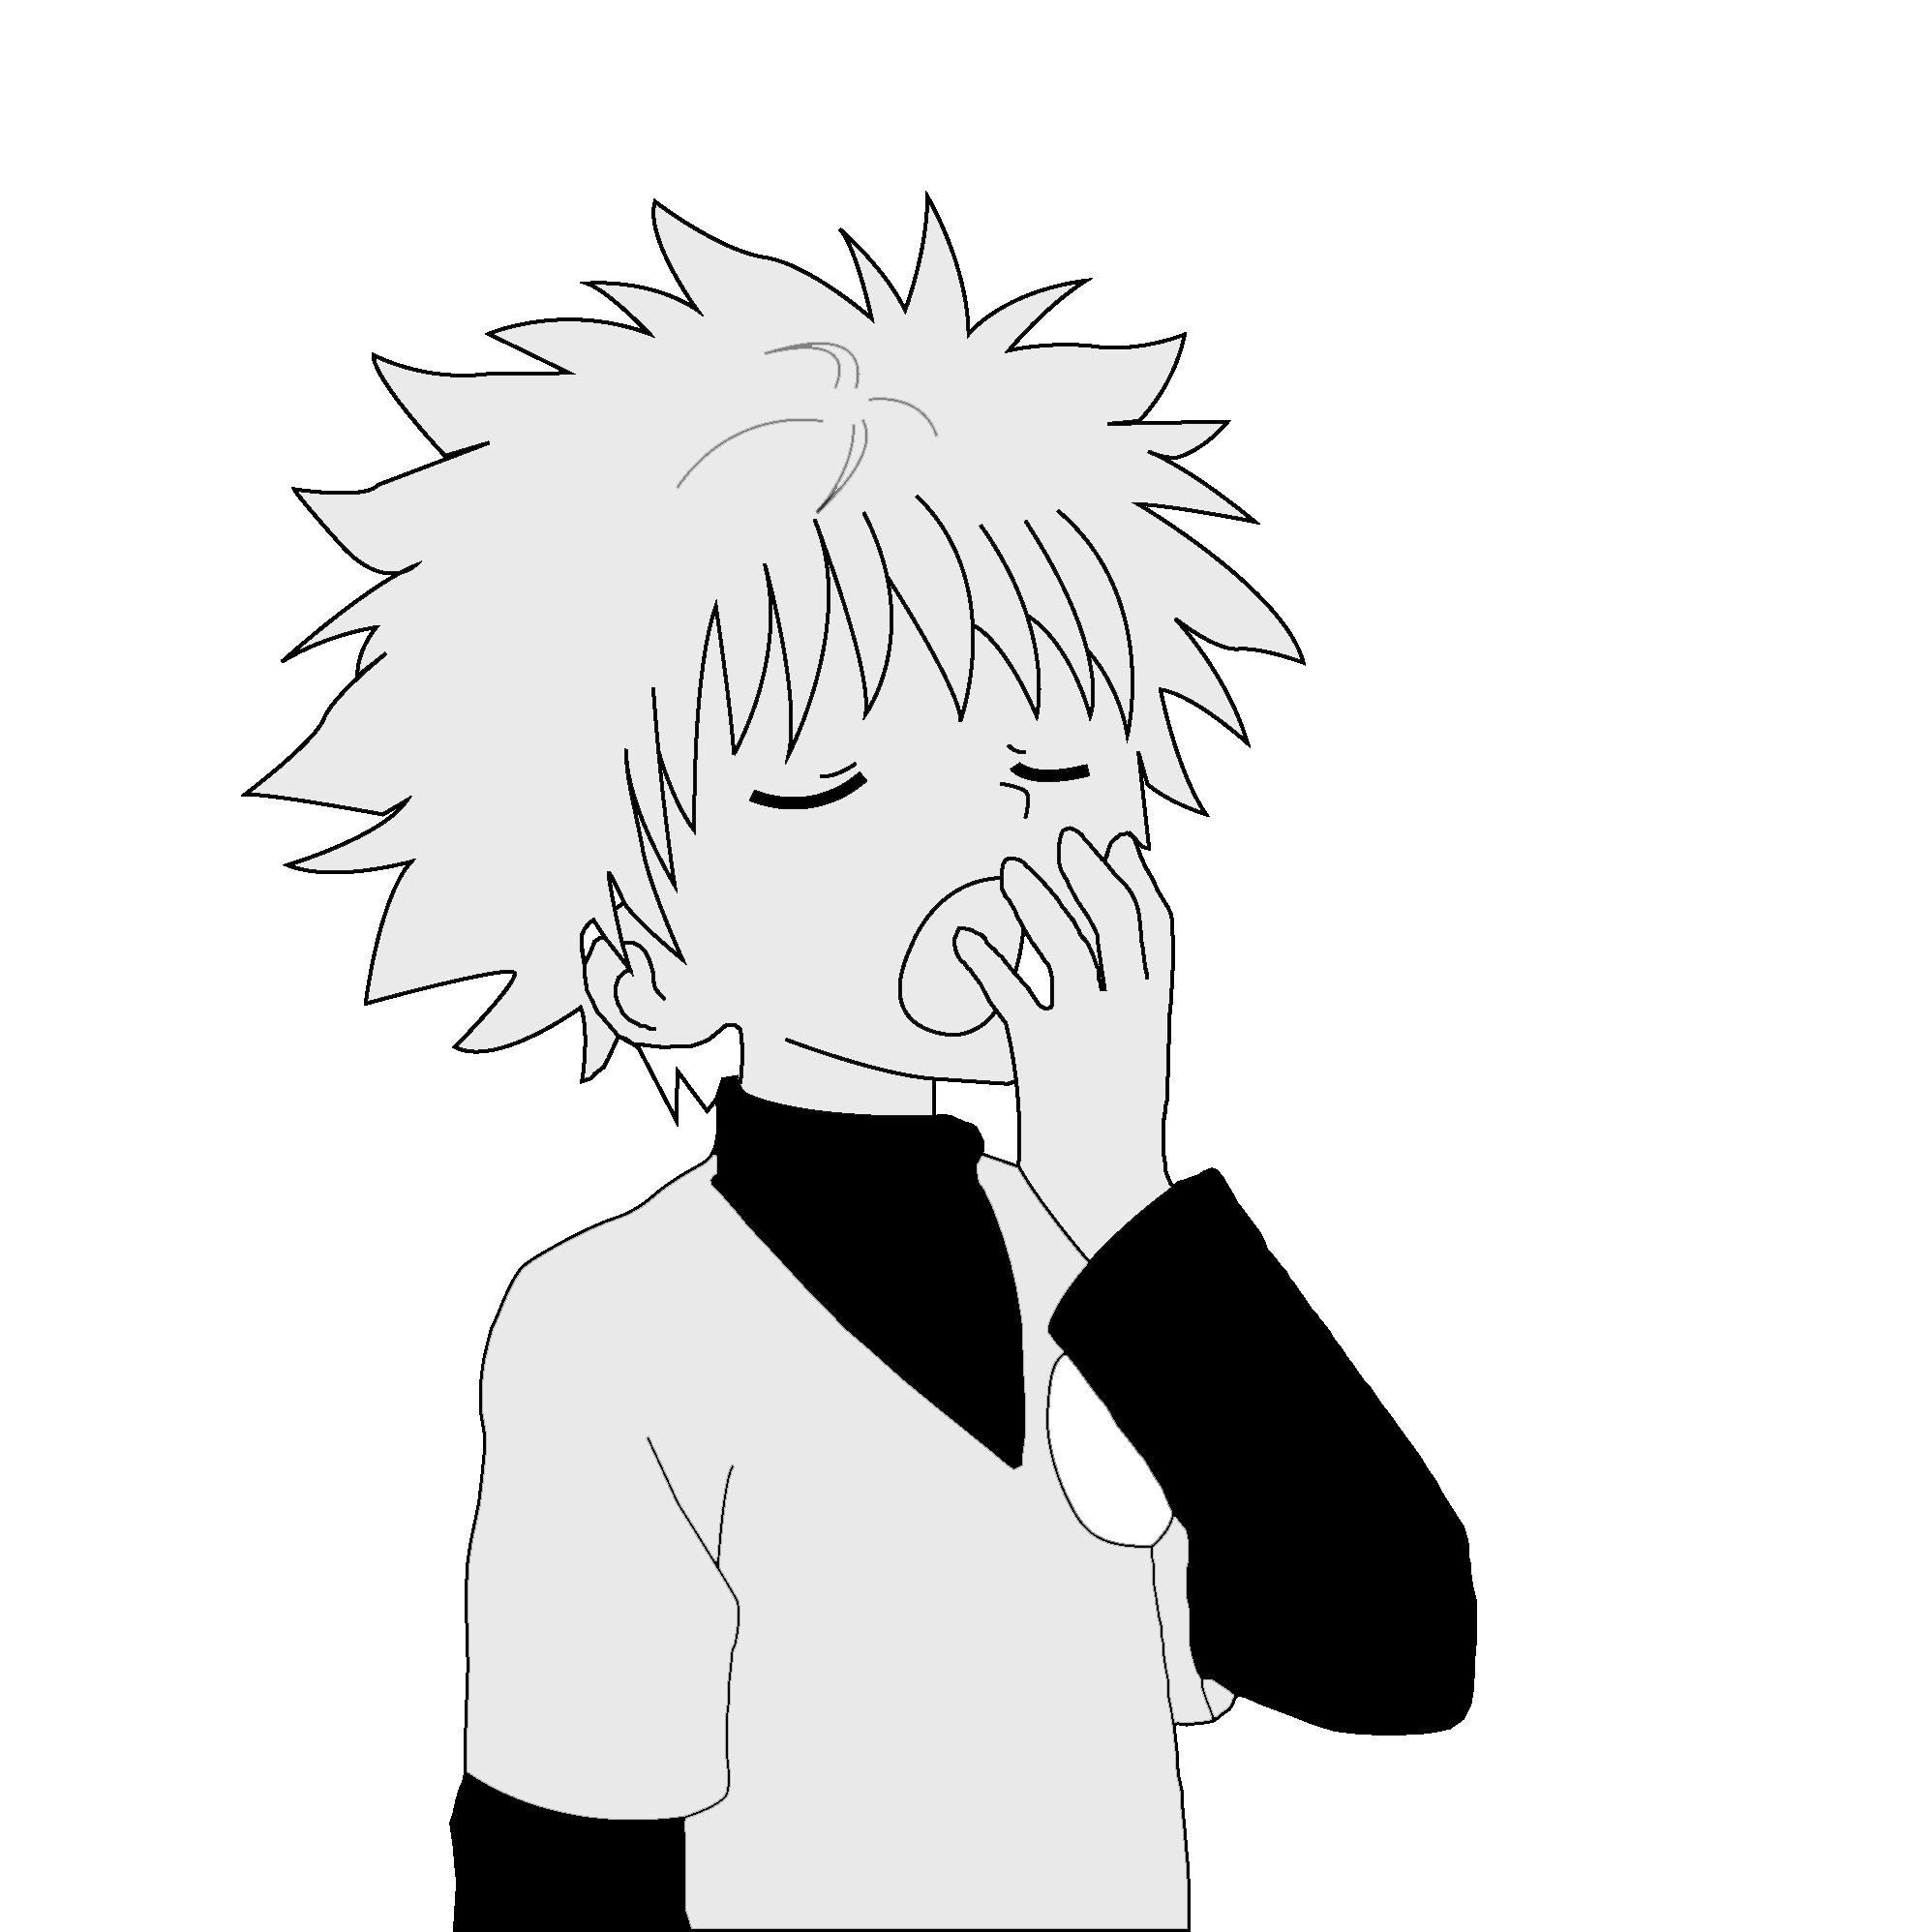
\includegraphics[width=.8em]{/Users/pluttan/Documents/bw2.png}}}}
\onehalfspacing

\pagestyle{fancy}
\renewcommand{\sectionmark}[1]{\markright{#1}}
\fancyhf{} 
\fancyhead[R]{\bfseries\thepage}
\fancyhead[LO]{\docopyright}

\newcommand{\image}[2]{
	\begin{figure}[H]
		\center{\includegraphics[height=#2pt]{../img/#1} }
    \end{figure}
}

\newcommand{\dotitle}[2]{

\thispagestyle{empty}
\sloppy{
  \scriptsize{
    \line(6,0){0}

    \centering \docopyright

    \centering Привет! Меня зовут Андрей, я создаю свою ботву, этот файл малая ее часть. 
    
    \centering Пользоваться и распространять файлы конечно же можно. Если вы нашли ошибку в файле, можете 
    
    \centering исправить ее в исходном коде и подать на слияние или просто написать в issue. 

    \centering {\bf{Так же вы можете купить распечатанную версию данного файла в виде книжки.}
    
    \centering По всем вопросам писать в ВК.}
    
    \centering Приятного бота)

    \line(6,0){300}

    \centering GitHub: \href{https://github.com/pluttan}

    \centering VK: \href{https://vk.com/pluttan}

    \line(6,0){0}
  }}

\begin{figure}[H]
		\center{\includegraphics[height=100pt]{/Users/pluttan/Documents/forMyDocs/qr2.png} }
\end{figure}

\topskip=-200pt
\vspace*{130pt}
\begin{Huge}
  \textbf{
    \begin{center}
        #1
    \end{center}
  }
  {\begin{center} 
        #2
    \end{center}}
\end{Huge}
\vspace*{300pt}
  \begin{flushright}
    Над файлом работали: \\
    \mycopyright
  \end{flushright}
\newpage
\pagestyle{fancy}
\renewcommand{\sectionmark}[1]{\markright{#1}}
\fancyhf{} 
\fancyhead[R]{\bfseries\thepage}
\fancyhead[LO]{\docopyright}
}
\renewcommand{\sectionmark}[1]{\markright{#1}}
\renewcommand{\sectionmark}[1]{\markright{#1}}
% \makeatletter
%      \renewcommand*\l@section{\@dottedtocline{1}{0em}{1.8em}}
%      \renewcommand*\l@subsection{\@dottedtocline{2}{1.5em}{2.0em}}
%      \renewcommand*\l@subsubsection{\@dottedtocline{3}{4.3em}{3.0em}}
% \makeatother
\newcommand{\toc}{
\newpage
\renewcommand{\contentsname}{Оглавление}
\large{\tableofcontents}
\newpage
\large
}


% It's XeLaTeX, if you can't compile comment this line 
\usepackage{fontspec}\setmainfont{Times New Roman} 


\newcommand{\bvec}[1]{\overrightarrow{#1}}
\newcommand{\mcol}[1]{\multicolumn{2}{c}{#1}}
\newcommand{\mcolt}[1]{&#1&}
\renewcommand{\a}{\vec{a}}
\renewcommand{\b}{\vec{b}}
\renewcommand{\c}{\vec{c}}
\renewcommand{\d}{\vec{d}}
\renewcommand{\i}{\vec{i}}
\renewcommand{\j}{\vec{j}}
\renewcommand{\k}{\vec{k}}
\newcommand{\nul}{\vec{0}}

\begin{document}

\dotitle{Подготовка к РК1}{Аналитическая геометрия}{}

\section{Базовые теоретические вопросы}

\subsection{Дать определение равенства геометрических векторов.}

Два вектора называются равными, если они сонаправлены и их длины равны.

\subsection{Дать определения суммы векторов и произведения вектора на число.}

\begin{center}
\begin{tabular}{c c} 
    \mcol{ Суммой двух векторов $\a$ и $\b$ называется такой вектор $\c$, 
    построенный по следующим правилам}\\
    Правило параллелограмма & Правило треугольника\\
    \mcol{Пусть $O$ любая точка.}\\
    \mcol{Отложим $\a$ от $O$. Получим $\bvec{OA}$.}\\
    \mcol{Отложим $\b$ от}\\
    Точки $O$ & Точки $A$\\
    \mcol{Получим}\\
\begin{minipage}[t]{0.4\linewidth}\image{1.png}{100}\end{minipage}&
\begin{minipage}[t]{0.4\linewidth}\image{2.png}{100}\end{minipage}\\
    \mcol{Построим}\\
    Параллелограмм & Треугольник\\
    \mcol{Вектор $\c$, представителем которого является $\bvec{OC}$ - искомый.}\\
    \mcol{Построение не зависит от выбора точки $O$ и правила построения.}\\\\
\end{tabular}
\end{center}

Произведением $\a$ на число $\alpha$ называется $\b$, если он коллинеарен $\a$
(причем если $\a \upuparrows \b: \ \alpha > 0$, иначе $\alpha < 0$ ) и его 
длина равна $|\alpha| |\a|$ 

\subsection{Дать определения коллинеарных и компланарных векторов.}

\begin{center}
\begin{tabular}{c c} 
    \mcol{Геометрические вектора называются}\\
    Коллинеарными & Компланарными\\
    \mcol{Если они лежат }\\
    На одной или параллельных прямых & На одной или параллельных плоскостях \\
\end{tabular}
\end{center}

\subsection{Дать определение линейно зависимой и линейно независимой системы векторов.}

\begin{center}
\begin{tabular}{c c} 
    \mcol{Векторы $\vec{a_1},...,\vec{a_n}$ называются линейно}\\
    Зависимыми & Независимыми\\
    Если существует & Если не существует\\
    \mcol{Их нетривиальная линейная комбинация, равная $\nul$, т.е.}\\
    \mcol{Если при $\alpha_1,...,\alpha_n \in \mathbb{R}, \ \alpha_1 \vec{a_1} +...+ \alpha_n \vec{a_n} = 0$ }\\
    $\exists \alpha_1,...,\alpha_n$ отличные от нуля & $\nexists \alpha_1,...,\alpha_n$ отличные от нуля \\
\end{tabular}
\end{center}

\subsection{Сформулировать геометрические критерии линейной зависимости 2-х и 3-х векторов.}

2 вектора линейно зависимы $\iff$ они коллинеарны

3 вектора линейно зависимы $\iff$ они компланарны

\subsection{Дать определение базиса и координат вектора.}

\begin{center}
\begin{tabular}{c c c} 
    \mcolt{Базисом в пространстве}\\
    $V_1$&$V_2$&$V_3$\\
    \mcolt{Называется}\\
    Любой ненулевой & Любая упорядоченная пара & Любая упорядоченная тройка\\
    вектор & коллинеарных векторов & некомпланарных векторов\\
    $\forall \vec{x} \in V_1 \exists ! x \in \mathbb{R}$&
    $\forall \vec{x} \in V_2 \exists ! x_1, x_2 \in \mathbb{R}$&
    $\forall \vec{x} \in V_3 \exists ! x_1, x_2, x_3 \in \mathbb{R}$\\
    $\vec{x} = x\vec{e}$ & $\vec{x} = x_1\vec{e_1} + x_2\vec{e_2}$ &
    $\vec{x} = x_1\vec{e_1} + x_2\vec{e_2} + x_3\vec{e_3}$\\
    \mcolt{Коэффициенты разложения}\\
    $x$&$x_1, x_2$&$x_1, x_2, x_3$\\
    \mcolt{Называются координатами $\vec{x}$ в базисе}\\
    $\vec{e}$&$\vec{e}_1, \vec{e}_2$&$\vec{e}_1, \vec{e}_2, \vec{e}_3$\\
\end{tabular}
\end{center}

\subsection{Сформулировать теорему о разложении вектора по базису.}

\begin{center}
Любой вектор можно разложить по базису, причем единственным способом
\begin{tabular}{c c c} 
    $\forall \vec{x} \in V_1 \exists ! x \in \mathbb{R}$&
    $\forall \vec{x} \in V_2 \exists ! x_1, x_2 \in \mathbb{R}$&
    $\forall \vec{x} \in V_3 \exists ! x_1, x_2, x_3 \in \mathbb{R}$\\
\end{tabular}
\end{center}

\subsection{Дать определение ортогональной скалярной проекции вектора на направление.}

Ортогональной проекцией вектора $\a$ на вектор $\b$ называется число, вычисленное по правилу:
\begin{enumerate}
    \item Отложим вектор $\a$ от любой точки $A$, получим $\bvec{AB}$
    \item Возьмем любую ось $b$, направление которой совпадает с $\b$
    \item Спроецируем $\bvec{AB}$ на $b$ и получим  $\bvec{A_{np}B_{np}}$
    \item Найдем число $\pm |\bvec{A_{np}B_{np}}|$, где $+$ если $\bvec{A_{np}B_{np}} \upuparrows \b$, иначе $-$
\end{enumerate}
Обозначение $np_{\b} \a$

\subsection{Дать определение скалярного произведения векторов.}

Скалярным произведением 2 векторов $\a$ и $\b$ называется число, равное произведению длин
векторов на косинус угла между ними.

\subsection{Сформулировать свойство линейности скалярного произведения.}

\begin{center}
$\forall \a, \b \forall k \in \mathbb{R}$

$(k\a)\b = k(\a\b)$

$\a(k\b) = k(\a\b)$\\

$\forall \a, \b, \c$

$(\a + \b)\c = \a\c + \b\c$

$\a(\b + \c) = \a\b + \a\c$
\end{center}

\subsection{Записать формулу для вычисления скалярного произведения двух векторов, заданных в ортонормированном базисе.}

$$\a\b = \a_1\b_1 + \a_2\b_2 + \a_3\b_3,
\a\{a_1;a_2;a_3\},\b\{b_1;b_2;b_3\} $$

\subsection{Записать формулу для вычисления косинуса угла между векторами, заданными в ортонормированном базисе.}

$$cos(\a,\b) = \frac{ \a \b }{ |\a| |\b| } = 
\frac{\a_1\b_1 + \a_2\b_2 + \a_3\b_3}
{\sqrt{\a_1 + \a_2 + \a_3}\sqrt{\b_1+\b_2+\b_3}}$$

\subsection{Дать определение правой и левой тройки векторов.}

\begin{center}
\begin{tabular}{c c} 

    \mcol{Упорядоченная тройка некомпланарных векторов $\a, \b, \c$ называется }\\
    Правой & Левой \\
    \mcol{Если кратчайший поворот от $\a$ к $\b$ виден из конца $\c$ проходящей}\\
    Против часовой стрелке & По часовой стрелке\\

\end{tabular}
\end{center}

\subsection{Дать определение векторного произведения векторов.}

Векторным произведением 2 векторов $\a$, $\b$ называется вектор $\c$, удовлетворяющих условиям
\begin{enumerate}
    \item $\c \perp \a, \c \perp \b$
    \item Упорядоченная тройка $\a$, $\b$, $\c$ правая
    \item $|\c| = |\a||\b|sin(\a, \b)$
\end{enumerate}

\subsection{Сформулировать свойство коммутативности (симметричности) скалярного произведения 
и свойство антикоммутативности (антисимметричности) векторного произведения.}

\begin{center}
$\forall \a, \b$

$\a\b = \b\a$ - симметричность скалярного произведения

$\a \times \b = - \b \times \a$ - кососимметричность векторного произведения
\end{center}

\subsection{Сформулировать свойство линейности векторного произведения векторов.}

\begin{center}
    $\forall \a, \b \forall k \in \mathbb{R}$
    
    $(k\a) \times \b = k(\a \times \b)$
    
    $\a \times (k\b) = k(\a \times \b)$\\
    
    $\forall \a, \b, \c$
    
    $(\a + \b) \times \c = \a \times \c + \b \times \c$
    
    $\a \times (\b + \c) = \a \times \b + \a \times \c$
\end{center}

\subsection{Записать формулу для вычисления векторного произведения в правом ортонормированном базисе.}

\begin{center}
$\a \times \b = 
\begin{vmatrix}
    \i&\j&\k\\
    a_1 & a_2 & a_3\\
    b_1 & b_2 & b_3
\end{vmatrix} = \i
\begin{vmatrix}
    a_2 & a_3\\
    b_2 & b_3
\end{vmatrix} - \j
\begin{vmatrix}
    a_1 & a_3\\
    b_1 & b_3
\end{vmatrix} + \k
\begin{vmatrix}
    a_1 & a_2\\
    b_1 & b_2
\end{vmatrix}, \a\{a_1;a_2;a_3\},\b\{b_1;b_2;b_3\}$
\end{center}

\subsection{Дать определение смешанного произведения векторов.}

Смешанным произведением 3 векторов $\a, \b, \c$ называется число, равное 
$(\a \times \b) \c$

Обозначение $(\a, \b, \c)$, $\a \b \c$

\subsection{Сформулировать свойство перестановки (кососимметричности) смешанного произведения.}

При перестановке любых двух векторов, смешанное произведение меняет знак.

$\forall \a, \b, \c:\a \b \c = - 
\b \a \c = - \c \b \a$

\subsection{Сформулировать свойство линейности смешанного произведения.}

\begin{center}
$\forall \a, \b, \c, \forall k \in \mathbb{R}$

$(k\a)\b\c = k(\a\b\c)$

$\a(k\b)\c = k(\a\b\c)$

$\a\b(k\c) = k(\a\b\c)$\\

$\forall \a, \b, \c, \d$

$(\a+\d)\b\c = \a\b\c + \d\b\c$

$\a(\b+\d)\c = \a\b\c + \a\d\c$

$\a\b(\c+\d) = \a\b\c + \a\b\d$
\end{center}

\subsection{Записать формулу для вычисления смешанного произведения в правом ортонормированном базисе.}

$$\a\b\c = 
\begin{vmatrix}
    a_1 & a_2 & a_3\\
    b_1 & b_2 & b_3\\
    c_1 & c_2 & c_3
\end{vmatrix} \ \a\{a_1;a_2;a_3\},
\b\{b_1;b_2;b_3\}, \c\{c_1;c_2;c_3\}$$

\subsection{Записать общее уравнение плоскости и уравнение «в отрезках». Объяснить 
геометрический смысл входящих в эти уравнения параметров.}

$$Ax + By + Cz + D = 0$$где $A, B, C$ - координаты вектора нормали плоскости $\vec{n}\{A, B, C\}$
$$\frac{x}{a}+\frac{y}{b}+\frac{z}{c} = 1$$a, b, c–соответствующие координаты точек 
лежащих на осях OX, OY и OZ соответственно.

\image{4.png}{200}


\subsection{Записать уравнение плоскости, проходящей через 3 данные точки.}
Пусть известны 3 точки $M_1(x_1,y_1,z_1),M_2(x_2,y_2,z_2),M_3(x_3,y_3,z_3)$
Тогда уравнение плоскости, которую они образуют будет равно 


$$
 \begin{cases}
   x = x_1+(x_2-x_1)u+(x_3-x_1)v\\
   y = y_1+(y_2-y_1)u+(y_3-y_1)v\\
   z = z_1+(z_2-z_1)u+(z_3-z_1)v\\
 \end{cases}
 u,v \in \mathbb{R}
$$

\subsection{Записать условия параллельности и перпендикулярности плоскостей.}

Пусть $\begin{cases}\pi_1: A_1x+B_1y+C_1z+D_1 = 0\\\pi_2: A_2x+B_2y+C_2z+D_2 = 0\end{cases}$
плоскости в пространстве, заданные в аффинной системе координат. Тогда 
\begin{enumerate}
    % \item $\pi_1 \equiv \pi_2 \iff \frac{A_1}{A_2} = \frac{B_1}{B_2} = \frac{C_1}{C_2} = \frac{D_1}{D_2}$
    \item $\pi_1 \parallel \pi_2 \iff \frac{A_1}{A_2} = \frac{B_1}{B_2} = \frac{C_1}{C_2} \ne \frac{D_1}{D_2}$
    % \item $\pi_1 \cap \pi_2 \iff \frac{A_1}{A_2} \ne \frac{B_1}{B_2}$ или $\frac{A_1}{A_2} \ne \frac{C_1}{C_2}$ или
    % $\frac{B_1}{B_2} \ne \frac{C_1}{C_2}$
    \item (Если система координат прямоугольная) $\pi_1 \perp \pi_2 \iff A_1A_2 + B_1B_2 + C_1C_2 = 0$
\end{enumerate} 


\subsection{Записать формулу для расстояния от точки до плоскости, заданной общим уравнением. }

$$\begin{cases}\pi: Ax+By+Cz+D = 0\\M_0(x_0,y_0,z_0)\end{cases}: \rho(M_0,\pi) = 
\frac{ |Ax_0+By_0+Cz_0+D| }{\sqrt{A^2+B^2+C^2}}$$

\subsection{Записать канонические и параметрические уравнения прямой в пространстве. 
Объяснить геометрический смысл входящих в эти уравнения параметров.}

Канонические 
$$ \frac{x-x_0}{a} = \frac{y-y_0}{b} = \frac{z-z_0}{c}$$

Параметрические
$$\begin{cases}x = x_0 + at\\y = y_0 + bt\\z = z_0 + ct\\\end{cases} t \in \mathbb{R}$$

Где $\vec{m}\{a,b,c\}$ направляющий вектор прямой, $M_0(x_0,y_0,z_0)$, точка
от которой отложен вектор $\vec{m}$

\image{5.png}{200}

\subsection{Записать уравнение прямой, проходящей через две данные точки в пространстве. }

$$\begin{cases}M_1(x_1,y_1,z_1)\\M_2(x_2,y_2,z_2)\end{cases}: 
\frac{x-x_1}{x_2-x_1} = \frac{y-y_1}{y_2-y_1} = \frac{z-z_1}{z_2-z_1}$$

\subsection{Записать условие принадлежности двух прямых одной плоскости.}

$l_1$(задан точкой $M_1$ и направляющим вектором $\vec{m}_1$) и $l_2$(Задан точкой $M_2$ и направляющим 
вектором $\vec{m}_2$) лежат в одной плоскости $\iff \bvec{M_1M_2}\vec{m_1}\vec{m_2} = 0$
Т.е. $\bvec{M_1M_2}, \vec{m}_1, \vec{m}_2$ компланарны. 

\subsection{Записать формулу для расстояния от точки до прямой в пространстве.}

Пусть $l_1$(задан точкой $M_1(x_1, y_1, z_1)$ и направляющим вектором $\vec{m}_1\{a,b,c\}$) и точка 
$M_0(x_0,y_0,z_0)$ тогда 
$$\rho(M_0, l_1) = \frac{ |\bvec{M_1M_0}\times\vec{m}| }{ |\vec{m}| } = 
\frac{\sqrt{\begin{vmatrix}y_0-y_1&z_0-z_1\\b&c\end{vmatrix}^2+
\begin{vmatrix}x_0-x_1&z_0-z_1\\a&c\end{vmatrix}^2+
\begin{vmatrix}x_0-x_1&y_0-y_1\\a&b\end{vmatrix}^2}}{\sqrt{a^2+b^2+c^2}}$$

\subsection{Записать формулу для расстояния между скрещивающимися прямыми.}

Пусть $l_1$(задан точкой $M_1(x_1, y_1, z_1)$ и направляющим вектором $\vec{m}_1\{a_1,b_1,c_1\}$) и 
$l_2$(Задан точкой $M_2(x_2, y_2, z_2)$ и направляющим вектором$\vec{m}_2\{a_2,b_2,c_2\}$)

$$\rho(l_1, l_2) = \frac{ |\bvec{M_1M_2}\vec{m_1}\vec{m_2}| }{ |\vec{m_1}\times\vec{m_2}| }=
\frac{ |\begin{vmatrix}x_2-x_1&y_2-y_1&z_2-z_1\\a_1&b_1&c_1\\a_2&b_2&c_2\end{vmatrix}| }
    {\sqrt{\begin{vmatrix}b_1&c_1\\b_2&c_2\end{vmatrix}^2+
    \begin{vmatrix}a_1&c_1\\a_2&c_2\end{vmatrix}^2+
    \begin{vmatrix}a_1&b_1\\a_2&b_2\end{vmatrix}^2}}$$

\section{Теоретические вопросы повышенной сложности}

\subsection{Доказать геометрический критерий линейной зависимости трёх векторов.}

3 вектора линейно зависимы $\iff$ они компланарны

\subsubsection{Необходимость}

Пусть $\a, \b, \c$ линейно зависимы, тогда один их них является линейной комбинацией
остальных. К примеру $\a = \beta\b + \gamma\c (\beta,\gamma \in \mathbb{R})$
Приложим $\a, \b, \c$ к одной точке $O$, получим $\bvec{OA}, \bvec{OB}, \bvec{OC}:$
$\bvec{OA} = \beta\bvec{OB} + \gamma\bvec{OC}$. Тогда $\bvec{OA}$ диагональ параллелограмма.
Следовательно $\bvec{OA}, \bvec{OB}, \bvec{OC}$ лежат в одной плоскости, значит они компланарны,
тогда и векторы $\a, \b, \c$ тоже компланарны.
\image{3.png}{200}

\subsubsection{Достаточность}

Пусть $\a, \b, \c$ комплонарны. Рассмотрим 2 случая:

1. Хотя бы один нулевой $(\a = \nul)$. Тогда $\a = \nul\b + \nul\c$
т.е. $\a$ является линейной комбинацией $\b, \c$ тогда по основной теореме
$\a, \b, \c$ линейно зависимы. 

2. Ни один не нулевой. Приложим $\a, \b, \c$ к одной точке $O$, 
получим $\bvec{OA}, \bvec{OB}, \bvec{OC}$, которые лежат в одной плоскости.
\image{3.png}{200}
$\bvec{OA} = \bvec{OB_1} + \bvec{OC_1}$. Т.к. $\bvec{OB}, \bvec{OB_1}$ коллинеарны, то
$\bvec{OB_1} = \beta\bvec{OB}$, аналогично $\bvec{OC_1} = \beta\bvec{OC}$ 
$\a = \beta\b + \gamma\c$, тогда $\a, \b, \c$ линейно зависимы.

\subsection{Доказать теорему о разложении вектора по базису.}

\begin{center}
Любой вектор можно разложить по базису, причем единственным способом
\begin{tabular}{c c c} 
    $\forall \vec{x} \in V_1 \exists ! x \in \mathbb{R}$&
    $\forall \vec{x} \in V_2 \exists ! x_1, x_2 \in \mathbb{R}$&
    $\forall \vec{x} \in V_3 \exists ! x_1, x_2, x_3 \in \mathbb{R}$\\
\end{tabular}
\end{center}

\subsubsection{Существование}

Из геометрических критериев следует, что 4 вектора $\vec{x}, \vec{e_1}, \vec{e_2}, \vec{e_3}$.
Тогда $\exists \alpha_0, \alpha_1, \alpha_2, \alpha_3$ (не все равны нулю), что
$\alpha_0\vec{x} + \alpha_1\vec{e_1} + \alpha_2\vec{e_2} + \alpha_3\vec{e_3} = \nul (1)$.
Тогда по определению линейно зависимых $\vec{e_1}, \vec{e_2}, \vec{e_3}$ линейно зависимы,
т.е. компланарны. $\vec{e_1}, \vec{e_2}, \vec{e_3}$ - базис в $V_3$ $\alpha_0 \ne 0$.
Умножим (1) на $\frac{1}{\alpha_0}$ и выразим $\vec{x}$. 
$\vec{x} = -\frac{\alpha_1}{\alpha_0}\vec{e_1}-\frac{\alpha_2}{\alpha_0}\vec{e_2}
-\frac{\alpha_3}{\alpha_0}\vec{e_3}$. Пусть $-\frac{\alpha_i}{\alpha_0} = x_i$, тогда
$\vec{x} = x_1\vec{e_1} + x_2\vec{e_2} + x_3\vec{e_3}$

\subsubsection{Единственность}

От противного. Пусть существуют 2 разложения для 
$\vec{x}: \vec{x} = x_1\vec{e_1} + x_2\vec{e_2} + x_3\vec{e_3};$
$\vec{x} = y_1\vec{e_1} + y_2\vec{e_2} + y_3\vec{e_3}$
Рассмотрим разность $\nul = \vec{x} - \vec{x} = 
(x_1 - y_1)\vec{e_1} + (x_2 - y_2)\vec{e_2} + (x_3 - y_3)\vec{e_3}$ - линейная комбинация 
$\vec{e_1}, \vec{e_2}, \vec{e_3}$. Т.к. $\vec{e_1}, \vec{e_2}, \vec{e_3}$ не компланарны
тогда их линейная комбинация равна $\nul$, $x_1 - y_1 = 0$ $x_2 - y_2 = 0$ $x_3 - y_3 = 0$
Получили $x_1 = y_1$ $x_2 = y_2$ $x_3 = y_3$ разложение единственно.

\subsection{Доказать свойство линейности скалярного произведения.}

\begin{center}
    $\forall \a, \b, \c \forall k \in \mathbb{R}$
\end{center}

\subsubsection{$(k\a)\b = k(\a\b)$}

1. $\b = \nul$ левая часть $ = (k\a)\nul = \nul$, правая часть $ = k(\a\nul) = \nul$

2. $\b \ne \nul$ левая часть $ = (k\a)\b = \b(k\a) = |\b|np_{\b}(k\a) =
k|\b|np_{\b}(\a) = k(\b\a) = k(\a\b) = $ правая часть

\subsubsection{$\a(k\b) = k(\a\b)$}

Левая часть $ = \a(k\b) = (k\b)\a = k(\a\b) = $ правая часть

\subsubsection{$(\a + \b)\c = \a\c + \b\c$}

1. $\c = \nul$ левая часть $ = (\a + \b)\c = \nul$, 
правая часть $ = \a\nul + \b\nul = \nul$

2. $\c \ne \nul$ левая часть $ = \c(\a + \b) = |\c|np_{\c}(\a + \b) =
|\c|(np_{\c}\a + np_{\c}\b) = \c\a + \c\b = 
\a\c + \b\c = $ правая часть

\subsubsection{$\a(\b + \c) = \a\b + \a\c$}

Левая часть $ = \a(\b + \c) = (\b + \c)\a = 
\a\b + \a\c = $ правая часть

\subsection{Вывести формулу для вычисления скалярного произведения векторов, заданных в ортонормированном базисе.}

$$\a\b = a_1b_1 + a_2b_2 + a_3b_3$$

Распишем по свойствам линейности $\a\b = (a_1\i + a_2\j + a_3\k)(b_1\i + b_2\j + b_3\k) = 
a_1b_1(\i\i) + a_1b_2(\i\j) + a_1b_3(\i\k) + a_2b_1(\j\i) + a_2b_2(\j\j) +a_2b_3(\j\k)+
a_3b_1(\k\i) + a_3b_2(\k\j) + a_3b_3(\k\k) = |\i\i=1,\i\j=0,\i\k=0,\j\j=1,\j\k=0,\k\k=0| = a_1b_1 + a_2b_2 + a_3b_3$

\subsection{Вывести формулу для вычисления векторного произведения в правом ортонормированном базисе.}

\begin{center}
$\a \times \b = 
\begin{vmatrix}
    \i&\j&\k\\
    a_1 & a_2 & a_3\\
    b_1 & b_2 & b_3
\end{vmatrix} = \i
\begin{vmatrix}
    a_2 & a_3\\
    b_2 & b_3
\end{vmatrix} - \j
\begin{vmatrix}
    a_1 & a_3\\
    b_1 & b_3
\end{vmatrix} + \k
\begin{vmatrix}
    a_1 & a_2\\
    b_1 & b_2
\end{vmatrix}, \a\{a_1;a_2;a_3\},\b\{b_1;b_2;b_3\}$
\end{center}

$\a \times \b = (a_1\i + a_2\j + a_3\k)\times(b_1\i + b_2\j + b_3\k)  = 
a_1b_1(\i\times\i) + a_1b_2(\i\times\j) + a_1b_3(\i\times\k) + a_2b_1(\j\times\i) + 
a_2b_2(\j\times\j) +a_2b_3(\j\times\k)+a_3b_1(\k\times\i) + a_3b_2(\k\times\j) + 
a_3b_3(\k\times\k) = |\i\times\i = \nul, \i\times\j = \k, \i\times\k = -\j, \j\times\i = -\k, 
\j\times\j = \nul, \j\times\k = \i, \k\times\i = \j, \k\times\j = -\i,\k\times\k = \nul|=
\i(\a_2\b_3+\a_3\b_2) + \j(\a_1\b_3+\a_3\b_1) + \k(\a_1\b_2+\a_2\b_1) = \i
\begin{vmatrix}
    a_2 & a_3\\
    b_2 & b_3
\end{vmatrix} - \j
\begin{vmatrix}
    a_1 & a_3\\
    b_1 & b_3
\end{vmatrix} + \k
\begin{vmatrix}
    a_1 & a_2\\
    b_1 & b_2
\end{vmatrix}  = 
\begin{vmatrix}
    \i&\j&\k\\
    a_1 & a_2 & a_3\\
    b_1 & b_2 & b_3
\end{vmatrix}$

\subsection{Доказать свойство линейности смешанного произведения.}

\begin{center}
    $\forall \a, \b, \c,\d \forall k \in \mathbb{R}$
\end{center}

\subsubsection{$(k\a)\b\c = k(\a\b\c)$}
$$(k\a)\b\c = ((k\a)\times\b)\c = (k(\a\times\b))\c = k((\a\times\b)\c) = k(\a\b\c)$$

\subsubsection{$\a(k\b)\c = k(\a\b\c)$}
$$\a(k\b)\c = (k\b)\c\a = k(\b\c\a) = k(\a\b\c)$$

\subsubsection{$\a\b(k\c) = k(\a\b\c)$}
$$\a\b(k\c) = (k\c)\a\b = k(\c\a\b) = k(\a\b\c)$$

\subsubsection{$(\a+\d)\b\c = \a\b\c + \d\b\c$}
$$(\a+\d)\b\c = ((\a+\d)\times\b)\c = (\a\times\b+\d\times\b)\c = \a\b\c+\d\b\c$$

\subsubsection{$\a(\b+\d)\c = \a\b\c + \a\d\c$}
$$\a(\b+\d)\c = (\b+\d)\c\a = \b\c\a + \d\c\a = \a\b\c + \a\d\c$$

\subsubsection{$\a\b(\c+\d) = \a\b\c + \a\b\d$}
$$\a\b(\c+\d) = (\c+\d)\a\b = \c\a\b+\d\a\b = \a\b\c + \a\b\d$$

\subsection{Вывести формулу для вычисления смешанного произведения трёх векторов в правом ортонормированном базисе.}

$$\a\b\c = (\a\times\b)\c = (\i
\begin{vmatrix}
    a_2 & a_3\\
    b_2 & b_3
\end{vmatrix} - \j
\begin{vmatrix}
    a_1 & a_3\\
    b_1 & b_3
\end{vmatrix} + \k
\begin{vmatrix}
    a_1 & a_2\\
    b_1 & b_2
\end{vmatrix})\c = c_1
\begin{vmatrix}
    a_2 & a_3\\
    b_2 & b_3
\end{vmatrix} - c_2
\begin{vmatrix}
    a_1 & a_3\\
    b_1 & b_3
\end{vmatrix} + c_3
\begin{vmatrix}
    a_1 & a_2\\
    b_1 & b_2
\end{vmatrix}  = 
\begin{vmatrix}
    a_1 & a_2 & a_3\\
    b_1 & b_2 & b_3\\
    c_1 & c_2 & c_3
\end{vmatrix}$$

\subsection{Вывести формулу для расстояния от точки до плоскости, заданной общим уравнением. }

$$\begin{cases}\pi:Ax + By + Cz + D =0\\M_0(x_0, y_0, z_0)\end{cases}:
    \rho (M_0, \pi) = \frac{ |Ax_0 + By_0 + Cz_0 + D| }{\sqrt{A^2+B^2+C^2}}$$

1. $\rho(M_0, \pi) = |\bvec{HM_0}|$, где $\bvec{HM_0}\{x_0-x_H,y_0-y_H,z_0-z_H,\}$

Пусть $\vec{n}$ - нормаль. Тогда $\vec{n}\bvec{HM_0} = |\vec{n}||\bvec{HM_0}|cos(\vec{n}, 
\bvec{HM_0}) = \pm|\vec{n}||\bvec{HM_0}| \rightarrow |\vec{n}\bvec{HM_0}| = 
|\vec{n}||\bvec{HM_0}|, |\bvec{HM_0}| = \frac{ |\vec{n}\bvec{HM_0}| }{ |\vec{n}| }$

2. Знаменатель $|\vec{n}| = \sqrt{A^2+B^2+C^2}$

3. Числитель $\vec{n}\bvec{HM_0} = A(x_0-x_H)+B(y_0-y_H)+C(z_0-z_H) = Ax_0 + By_0 
+ Cz_0 - (Ax_H + By_H + Cz_H) = Ax_0 + By_0 + Cz_0 + D$

4. $|\bvec{HM_0}| = \rho (M_0, \pi) = \frac{ |Ax_0 + By_0 + Cz_0 + D| }{\sqrt{A^2+B^2+C^2}}$

\subsection{Вывести формулу для расстояния от точки до прямой в пространстве.}

Пусть $l_1$(задан точкой $M_1(x_1, y_1, z_1)$ и направляющим вектором $\vec{m}_1\{a,b,c\}$) и точка 
$M_0(x_0,y_0,z_0)$ тогда 
$$\rho(M_0, l_1) = \frac{ |\bvec{M_1M_0}\times\vec{m}| }{ |\vec{m}| } = 
\frac{\sqrt{\begin{vmatrix}y_0-y_1&z_0-z_1\\b&c\end{vmatrix}^2+
\begin{vmatrix}x_0-x_1&z_0-z_1\\a&c\end{vmatrix}^2+
\begin{vmatrix}x_0-x_1&y_0-y_1\\a&b\end{vmatrix}^2}}{\sqrt{a^2+b^2+c^2}}$$

1. Рассмотрим параллелограмм построенный на  $\bvec{M_1M_0}$ и $\vec{m}$
$\rho(M_0, l_1) = h$, где $h$ высота параллелограмма.
$h = \frac{S}{ |\vec{m}| } = \frac{ |\bvec{M_1M_0} \times \vec{m}| }{ |\vec{m}| }$

2. Знаменатель $|\vec{m}| = \sqrt{a^2+b^2+c^2}$

3. Числитель $|\bvec{M_1M_0} \times \vec{m}| = |\begin{vmatrix}\i&\j&\k\\x_0-x_1&y_0-y_1&z_0-z_1\\a&b&c\end{vmatrix}| = 
|\begin{vmatrix}y_0-y_1&z_0-z_1\\b&c\end{vmatrix}\i-
\begin{vmatrix}x_0-x_1&z_0-z_1\\a&c\end{vmatrix}\j+
\begin{vmatrix}x_0-x_1&y_0-y_1\\a&b\end{vmatrix}\k|=
\sqrt{\begin{vmatrix}y_0-y_1&z_0-z_1\\b&c\end{vmatrix}^2+
\begin{vmatrix}x_0-x_1&z_0-z_1\\a&c\end{vmatrix}^2+
\begin{vmatrix}x_0-x_1&y_0-y_1\\a&b\end{vmatrix}^2}$

4.$h = \rho(M_0, l_1) = \frac{ |\bvec{M_1M_0}\times\vec{m}| }{ |\vec{m}| } = 
\frac{\sqrt{\begin{vmatrix}y_0-y_1&z_0-z_1\\b&c\end{vmatrix}^2+
\begin{vmatrix}x_0-x_1&z_0-z_1\\a&c\end{vmatrix}^2+
\begin{vmatrix}x_0-x_1&y_0-y_1\\a&b\end{vmatrix}^2}}{\sqrt{a^2+b^2+c^2}}$

\subsection{Вывести формулу для расстояния между скрещивающимися прямыми.}

Пусть $l_1$(задан точкой $M_1(x_1, y_1, z_1)$ и направляющим вектором $\vec{m}_1\{a_1,b_1,c_1\}$) и 
$l_2$(Задан точкой $M_2(x_2, y_2, z_2)$ и направляющим вектором$\vec{m}_2\{a_2,b_2,c_2\}$)

$$\rho(l_1, l_2) = \frac{ |\bvec{M_1M_2}\vec{m_1}\vec{m_2}| }{ |\vec{m_1}\times\vec{m_2}| }=
\frac{ |\begin{vmatrix}x_2-x_1&y_2-y_1&z_2-z_1\\a_1&b_1&c_1\\a_2&b_2&c_2\end{vmatrix}| }
    {\sqrt{\begin{vmatrix}b_1&c_1\\b_2&c_2\end{vmatrix}^2+
    \begin{vmatrix}a_1&c_1\\a_2&c_2\end{vmatrix}^2+
    \begin{vmatrix}a_1&b_1\\a_2&b_2\end{vmatrix}^2}}$$

1. Рассмотрим параллелепипед, построенный на $\bvec{M_1M_2}, \vec{m_1}, \vec{m_2}$
Пусть $\pi_1$ и $\pi_2$ плоскости нижнего и верхнего оснований, тогда $\rho(l_1, l_2) = h$ параллелепипеда
$h = \frac{V}{S} = \frac{ |\bvec{M_1M_2}\vec{m_1}\vec{m_2}| }{ |\vec{m_1}\times\vec{m_2}| }$

2.Числитель $|\bvec{M_1M_2}\vec{m_1}\vec{m_2}| =  |\begin{vmatrix}x_2-x_1&y_2-y_1&z_2-z_1\\
a_1&b_1&c_1\\a_2&b_2&c_2\end{vmatrix}|$

3. Знаменатель $|\vec{m_1}\times\vec{m_2}| = |\begin{vmatrix}
    \i&\j&\k\\
    a_1 & a_2 & a_3\\
    b_1 & b_2 & b_3
\end{vmatrix}| = |\i
\begin{vmatrix}
    a_2 & a_3\\
    b_2 & b_3
\end{vmatrix} - \j
\begin{vmatrix}
    a_1 & a_3\\
    b_1 & b_3
\end{vmatrix} + \k
\begin{vmatrix}
    a_1 & a_2\\
    b_1 & b_2
\end{vmatrix}| = $ \\
$=\sqrt{\begin{vmatrix}b_1&c_1\\b_2&c_2\end{vmatrix}^2+
\begin{vmatrix}a_1&c_1\\a_2&c_2\end{vmatrix}^2+
\begin{vmatrix}a_1&b_1\\a_2&b_2\end{vmatrix}^2}$

4. $h = \rho(l_1, l_2) = \frac{ |\bvec{M_1M_2}\vec{m_1}\vec{m_2}| }{ |\vec{m_1}\times\vec{m_2}| }=
\frac{ |\begin{vmatrix}x_2-x_1&y_2-y_1&z_2-z_1\\a_1&b_1&c_1\\a_2&b_2&c_2\end{vmatrix}| }
    {\sqrt{\begin{vmatrix}b_1&c_1\\b_2&c_2\end{vmatrix}^2+
    \begin{vmatrix}a_1&c_1\\a_2&c_2\end{vmatrix}^2+
    \begin{vmatrix}a_1&b_1\\a_2&b_2\end{vmatrix}^2}}$

\end{document}